\documentclass{article} % For LaTeX2e
\usepackage{nips15submit_e,times}
\usepackage{hyperref}
\usepackage{url}
\usepackage{graphicx}
%\documentstyle[nips14submit_09,times,art10]{article} % For LaTeX 2.09


\title{Classifying Arrhythmia using Deep Neural Networks}


\author{
Siddarth Sampangi \\
College of Information and Computer Sciences\\
University of Massachusetts, Amherst\\
Amherst, MA 01003 \\
\texttt{ssampangi@cs.umass.edu} \\
}

% The \author macro works with any number of authors. There are two commands
% used to separate the names and addresses of multiple authors: \And and \AND.
%
% Using \And between authors leaves it to \LaTeX{} to determine where to break
% the lines. Using \AND forces a linebreak at that point. So, if \LaTeX{}
% puts 3 of 4 authors names on the first line, and the last on the second
% line, try using \AND instead of \And before the third author name.

\newcommand{\fix}{\marginpar{FIX}}
\newcommand{\new}{\marginpar{NEW}}

\nipsfinalcopy % Uncomment for camera-ready version

\begin{document}


\maketitle

\begin{abstract}
Cardiac arrhythmia refers to any abnormality in beating of the heart. There are many types of cardiac arrhythmia ranging in severity, including premature beats, atrial fibrillation, and ventricular fibrillation. While arrhythmia classification has been well researched, this study focuses on the use of recent techniques in deep learning to classify arrhythmia with minimal possible data pre-processing. Using convolutional neural networks and long short-term memory recurrent neural networks, we were able to produce accuracies of 99.15\% and 98.59\% respectively.

\end{abstract}

\section{Introduction}
Electrocardiograms (ECG) are a popular, non-invasive tool used to monitor the beating of the heart. By observing the ECG waveforms of a heartbeat, diagnosis of abnormalities is possible. Cardiac arrhythmia is a general term for any abnormality in the rhythm or beat of the heart. The types of arrhythmia range in severity, with the most dangerous forms being life-threatening. The large number of patients in hospitals and the need to continuously monitor them motivates the investigation of automated arrhythmia detection systems. This area has been researched for the past 1-2 decades, with techniques ranging from hardware-level signal processing systems to more general algorithms using multi-layer perceptrons (MLP). In this work, we examine the performance of recently popularized neural network architectures on this task. While prior work on using MLPs for this task was still restricted to using very few hidden units, recent advancements in using graphics processing units (GPU) allows us to efficiently train networks with millions of units. Using convolutional neural networks and long short-term memory networks, we were able to achieve a test accuracy of 99.15\% and 98.59\%, respectively.

\section{Related work}
Gao et al. \cite{Gao} compare the performance of several methods such as naive bayes, decision trees, logistic regression, radial basis function networks, and bayesian artificial neural networks on the UCI arrhythmia data set, which provides incomplete data and includes patient information (such as age and weight) in addition to the standard ECG data. Their best results were obtained with a MLP with a dense layer with 10 units. Vishwa et al. \cite{Vishwa} used the MIT-BIH data set and trained a 3 layer MLP with 5 units in the first hidden layer and 3 in the second, and achieved a classification accuracy of 96.21\%. While they used far fewer hidden units and achieved only a slightly lower test accuracy compared to our networks, they performed additional preprocessing to their data by using a high-pass filter to reduce noise, and recent hardware advancements have mitigated the costs of using many hidden units such there are minimal advantages to using very few hidden units - our networks take less than 2 seconds to train a full epoch. Mohammadzadeh-Asl and Setarehdan \cite{Babak} use the MIT-BIH data set and the Creighton University Ventricular Tachyarrhythmia Database and train an MLP with one hidden layer consisting of 20 units to classify between 4 types of arrhythmia and normal heartbeats. They achieved a test accuracy of 99.38\% after performing extensive preprocessing and adding 11 new features to explicitly convey characteristics from the time and frequency domains to the network. Note that this is the only work we have found which achieves a classification accuracy that surpasses that of our own. While many others \cite{Ramirez} \cite{Nashash} \cite{Mitra} have studied this problem, none have explored the particular architectures that we do, and all fail to achieve better accuracy.

\section{Network architectures}
In this section, we shall provide a brief introduction to convolutional neural networks (CNN) and Long Short-Term Memory (LSTM) networks. These two types of networks are themselves variants of a general class of discriminative classifier called artificial neural networks (ANN). The atomic unit of the ANN is called a neuron. A neuron can receive inputs from any number of real-valued signals, and it produces a real-valued output by taking the inner product of its inputs with a weight matrix $W$, adding a bias $b$, and then passing the result to a nonlinear function. Multiple neurons that each receive identical copies of the input form a layer, and a basic ANN is formed by stacking layers such that the output of the $i^{th}$ layer is the input of the $(i+1)^{th}$ layer. 

An ANN is trained via stochastic gradient descent (SGD) over a loss function (usually some form of a difference taken between the true label and prediction) with respect to the $W$ matrix and bias $b$ of each neuron. To accomplish this, we use the backpropagation algorithm to localize dependencies so that, given a loss function $L$, we can easily calculate the gradient $\frac{\partial L}{\partial W_{i}}$ of the weights of a neuron $i$ given the gradients $\frac{\partial L}{\partial W_{j}}$ of the weights of all neurons $j$ that $i$ outputs to. Thus, the backpropagation algorithm calculates the gradients with respect to the final layer of the network, and then propagates the gradient to each preceding layer, minimizing the gradient at each layer with respect to the loss. For this to work, it is necessary for the nonlinearity used by each neuron to be differentiable. 

\subsection{Convolutional neural networks}
Convolutional networks are designed to exploit the spatial dependencies between units of an input. For example, an image of a flower is recognized as an image of a flower not only because of the RGB values of each pixel, but also because of the position of each pixel in relation to the surrounding pixels. Randomly scrambling the pixel locations in an image of a flower would result in an image that can no longer be recognized. As such, valuable information could exist in the order that an input is presented to the network. Currently, a vanilla ANN would output the same value regardless of the order of its inputs ($W_{1}x+W_{2}y = W_{2}y+W_{1}x$). 

A one dimensional convolution operation involves a filter of size $F$, an input of size $N$, a stride of size $S$, and a padding of size $P$. A convolution is performed by mirroring the filter across its axis, and using it as a sliding window over the input, at each step taking the inner product of the filter with the units of the input that the filter's window resides over at that step. The stride $S$ dictates how many input units to skip at each step, and the padding $P$ dictates the number of zero-padding units that are appended to both ends of the input. Since convolving a filter of size $x$ with an input of size $y$ results in an output of size $y-x+1$, padding is used to ensure a fixed output size. Thus, the overall formula for calculating output size is $\frac{N-F+2P}{S}+1$. 1D convolution can be trivially extended to 2D. 

Intuitively, a convolution of a filter over an image can be understood as an operation where the filter checks for the presence or response of a specific signal $G$ in the image. This response will be maximal when the filter's window lies directly over the signal it is trained to respond to. Thus, the output of a convolution can be seen as a sort of heatmap of the likelihood of the presence of $G$ at each point in the image. 

A convolutional layer is specified by the number of filters it contains, and the size, stride, and padding (usually common across all filters in a layer) of each filter. The input to the layer is supplied to every filter, and the output of each filter is stacked and outputted to the next layer. A CNN is typically comprised of one or more convolutional layers, followed by one or more dense layers. A dense layer contains neurons that each receive the entire input of the layer.

\subsection{LSTM networks}

While convolutional layers address dependencies between units of the same input, recurrent layers address inter-input dependencies. A major disadvantage of CNNs is their inability to process sequences of inputs jointly. That is, a CNN will always generate the same output for a given input regardless of previous inputs - a disadvantage when there are strong dependencies between inputs. Question-answer systems are an example of this. Considering words or characters as individual inputs, a CNN cannot process a question (or more generally, a phrase) because it considers each word separately. Supplying the entire phrase as a single input could solve this problem, but CNNs also take fixed length inputs (and produce fixed length outputs). This imposes a hard limit on the length of the question and answer, which is impractical. Recurrent neural networks (RNN) solve both of these problems by introducing the concept of memory. By maintaining an internal state, a RNN can process sequences of arbitrary length and produce outputs that depend on its entire history of inputs. If a CNN is trained as a one-to-one (one output for every input) network, a RNN can also be trained as a many-to-one, one-to-many, or many-to-many network.

A RNN represents memory by adding the (pre-activation function) output of every hidden unit in a layer as input to each hidden unit in that layer at the next time step. That is, while a hidden unit in an ANN only takes the previous layer's output as input, a hidden unit in a RNN uses the previous layer's output, as well as the output of all units in its layer from the previous time step. While there are no explicit links more than 1 time step into the past, the output of any time step is still dependent on all past outputs because each of those outputs has been used to calculate the output at the next time step, and so by induction, they have affected all future outputs.

While each output can theoretically affect all future outputs, in practice, the gradients of the network weights have been known to either vanish (approach 0) or explode. This is known as the vanishing gradient problem \cite{Hochreiter}, and generally, it is hard for a RNN to train on sequences where dependencies between inputs more than 10 time steps apart need to be learned \cite{Graves}. 

To this end, Hochreiter et. al. created Long Short-Term Memory RNNs \cite{LSTM}(LSTM). A LSTM consists of a cell that is used as memory, and 3 gates that control the flow of information through the gate. An input and output gate control the flow of information (at the current time step) into and out of the cell respectively. A forget gate allows the LSTM to 'clear' its memory. Each gate receives input from the layer input, the pre-activation function output of the current layer at the previous time step, and all cell states at the previous time step. The weights of each of those connections are learned through backpropagation. Since an LSTM can close its input gates, it can maintain its memory from any time step for an arbitrary number of time steps. 

\section{Data preprocessing}
We perform the minimal necessary preprocessing to the data. The MIT-BIH Arrhythmia Database \cite{Moody}, found on PhysioNet \cite{physionet}, consists of 48 two-channel ambulatory ECG recordings from patients, each a little over 30 minutes long, and digitized at 360 Hz per channel with 11-bit resolution over a 10 mV range.

For our purposes, the most general purpose algorithm would be able to process and classify the heartbeats in the original format they were recorded in (as 48 separate sequences). While this is ideal, we want to avoid enforcing dependencies between the labels of sequential heartbeats. Since all of the 48 sequences contain largely the same class of heartbeat (either a majority of normal heartbeats, or a majority of abnormal heartbeats), enforcing a heartbeat-to-heartbeat independence would be impossible if the networks were trained on the original (non-randomized) sequences. We could also have trained the networks on randomized versions of the sequences, where each heartbeat of a training sequence is sampled uniformly from all heartbeats across all of the original sequences, but that introduces another set of problems, such as the need to normalize all heartbeats to have the same baseline. Thus, we decided to train our networks on each individual heartbeat.

To define and extract a single heartbeat from a continuous ECG sequence, we decided to extract a series of samples centered around the R peak of the heartbeat, since that would likely contain all relevant features. Since each heartbeat is annotated at its R peak, the only parameter we needed to decide on was the size of the window that we would extract. We determined empirically that the average distance between two R peaks was approximately 0.75 seconds, and so we decided on a window size of 1.0 seconds to allow for a margin of error. Thus, given our dataset's constraints, we performed the minimal preprocessing.

A window size of 1 second led to nearly all examples containing 361 samples. 176 examples contained 360 samples, and to simplify their processing in the  networks, we simply duplicated the last sample to allow a uniform sample size for each heartbeat. Exactly 100 annotated heartbeats could not be used as examples because their R peaks are too close (within 0.5 seconds) to either the beginning of their respective sequence or the end.

Starting with 110631 examples, we removed the 100 examples that did not contain the full 361 samples. We also removed the examples for which the annotation was neither 'normal' or some type of arrhythmia. Examples include paced heartbeats, ventricular flutter waves, unclassifiable heartbeats, and heartbeats that are a fusion of normal and paced or normal and ventricular. After removing these irrelevant examples, we had a set of 93521 examples, of which 18482 (19.7\%) are indicative of arrhythmia.

Taking a random 80/20 split for the training and test sets, and subsampling the 'normal' examples to allow a 50/50 split between examples of arrhythmia and examples of normal beats, we have a training set of 29572 examples, and a test set of 7392 examples.

\section{Experiments and Results}
We trained several CNN and LSTM architectures and settled on a base architecture for each on which we ran our experiments. The CNN we used was comprised of an initial convolutional layer with 50 filters, each of size (30,1), followed by a maxpool layer of size (5,1), a fully-connected layer with 100 units, and finally a sigmoid layer with 1 unit. The LSTM was comprised of an LSTM layer with 30 units, a fully-connected layer with 100 units, and a sigmoid layer with 1 unit. We trained both networks with 50\% dropout on their respective fully-connected layers, as dropout is known to be less helpful on LSTM and convolutional layers. We briefly experimented with increasing the number of layers, their respective sizes, or the dropout probability on each network, and did not notice a definite increase in performance. We believe that the proposed architecture is sufficient due to the relative simplicity of the dataset. Apart from the regularization lambda, hyperparameters were also fixed to constants that are known to be reasonable in practice. We initialized our learning rate to 0.01, and decremented it by $\frac{0.01-0.001}{1500} = 6 \times 10^{-6}$ at each of the 1500 epochs. Validation error stopped improving well before 1500 epochs for all of our experiments, so further training would not have improved our results. Lastly, we used Nesterov momentum \cite{Sutskever} to update the network weights, and set the momentum to 0.9.

Training was performed with batch stochastic gradient descent (SGD) with a batch size of 256. We used cross entropy for our loss function and L2 regularization, where our experiments tested values of the regularization coefficient $\lambda$. Initial tests showed that setting $\lambda$ to over 0.01 resulted in a significant drop in performance, so we tested uniformly spaced values in the range [0,0.01] ie. 0.0, 0.001, 0.002,..., 0.01. We used 4-fold cross-validation, and show the average validation accuracies per epoch over all values of $\lambda$ in Figure 1. Note that the data points are well stratified in inverse order of their respective $\lambda$ values, which further corroborates the conclusion that the best value for $\lambda$ is 0.0.

\begin{figure}[h]
\centering
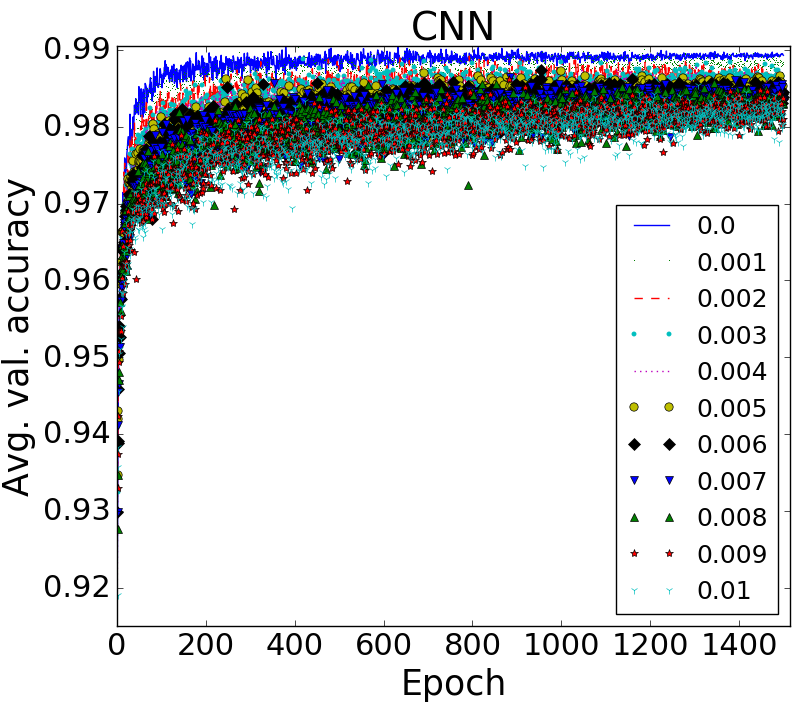
\includegraphics[scale=0.34]{media/CNNPerformance.png}
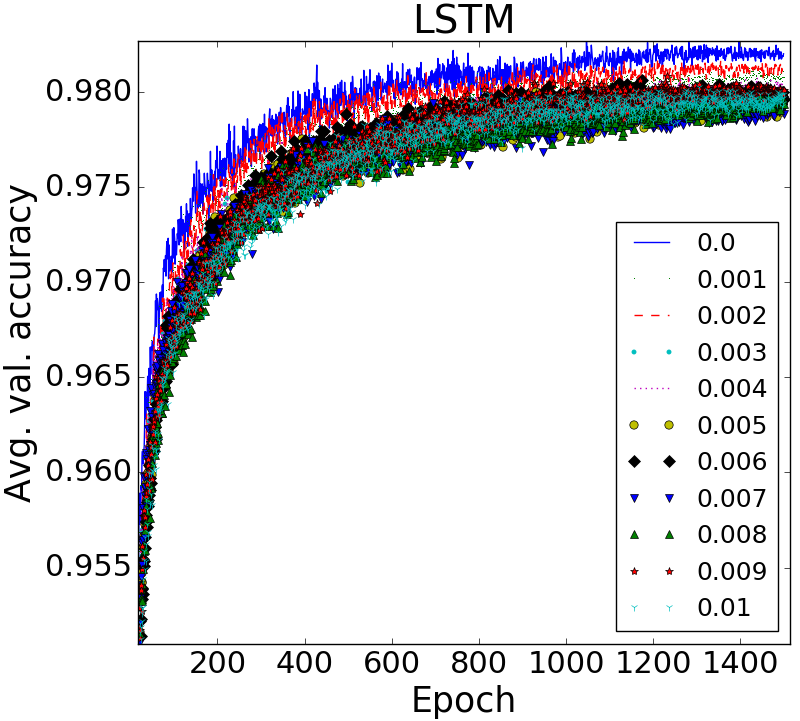
\includegraphics[scale=0.33]{media/LSTMPerformance.png}
\caption{Average validation accuracies of each network per given $\lambda$. Each data point represents the average validation accuracy over a 4-fold cross-validation scheme after training for the given number of epochs and using the given value for $\lambda$.}
\end{figure}

With a $\lambda$ of 0.0, we trained a CNN and an LSTM on the entire dataset and achieved test accuracies of 99.15\% and 98.59\% respectively.

\section{Conclusion and Future Work}

In this work, we evaluated the performance of CNNs and LSTMs on diagnosing cardiac arrhythmia. With the exception of one other work which partially uses a separate data set for reporting test performance, our systems have achieved a test accuracy that surpasses that of any other work we know of, despite avoiding virtually all forms of preprocessing or specialization to the current problem. While we achieved good performance, this project mainly served as a proof-of-concept for targetting arrhythmia classification with deep architectures. Interesting areas for further investigation include multi-class classification, a more fine-grained search over the hyperparameter space, and experiments with other types of models such as autoencoders and restriced boltzmann machines. Furthermore, we have deliberately avoided extensive preprocessing in this work to gain insight on the basic capabilities of CNNs and LSTMs. Focusing purely on improving the test accuracies of our networks, experimenting on with various preprocessing techniques could produce better results. Lastly, as mentioned before, data from the MIT-BIH dataset prevents us from approaching this task as a true sequence-to-sequence problem. If sequences of continuous heartbeats (ie. a record from a single person) can be found which contain both normal and abnormal beats, we could test our networks in a far more realistic setting by passing them sequences of multiple beats at a time.

\begin{thebibliography}{9}

\bibitem{Gao}
Gao, D.; Madden, M.; Chambers, D.; Lyons, G.; Bayesian ANN Classifier for ECG Arrhythmia Diagnostic System: A Comparison Study. International Joint Conference on Neural Networks. 2005.

\bibitem{Vishwa}
Vishwa, A.; Lal, M.; Dixit, S.; Vardwaj, P.; Clasification Of Arrhythmic ECG Data Using Machine Learning Techniques. International Journal of Interactive Media and Artificial Intelligence. 2011.

\bibitem{Babak}
 Mohammadzadeh-Asl, B.; Setarehdan, S.; Neural network based arrhythmia classification using heart rate variability signal. European Signal Processing Conference. 2006.

\bibitem{Ramirez}
Ramirez, E.; Castillo, O.; Soria, J.; Hybrid System for Cardiac Arrhythmia Classification with Fuzzy K-Nearest Neighbors and Neural Networks Combined by a Fuzzy Inference System. Soft Computing for Recognition Based on Biometrics. pp 37-55. Print. 2010.

\bibitem{Nashash}
Al-Nashash, H.; Cardiac arrhythmia classification using neural networks; Technology and Healthcare. pp 363-372. 2000.

\bibitem{Mitra}
Mitra, M.; Samanta, R.K.; Cardiac arrhythmia classification using neural networks with selected features. First International Conference on Computational Intelligence: Modeling Techniques and Applications. 2013.

\bibitem{Hochreiter}
Hochreiter, S.; Bengio, Y.; Frasconi, P.; and Schmidhuber, J.; Gradient flow in recurrent nets: the difficulty of learning long-term dependencies. In S. C. Kremer and J. F. Kolen, editors, A Field Guide to Dynamical Recurrent Neural Networks. IEEE Press, 2001.

\bibitem{Graves}
Graves, A.; Supervised Sequence Labelling with Recurrent Neural Networks. 2012. \textit{PhD Thesis}

\bibitem{LSTM}
Hochreiter, S.; Schmidhuber, J.; Long Short-Term Memory. Neural Computation, 9(8):1735–1780, 1997.

\bibitem{Moody} 
Moody, GB; Mark, RG.; The impact of the MIT-BIH Arrhythmia Database. \textit{IEEE Eng in Med and Biol} 20(3):45-50 (May-June 2001). (PMID: 11446209)
 
\bibitem{physionet} 
Goldberger, AL; Amaral, LAN; Glass, L; Hausdorff, JM; Ivanov, PCh; Mark, RG; Mietus, JE; Moody, GB; Peng, C-K; Stanley, HE.; PhysioBank, PhysioToolkit, and PhysioNet: Components of a New Research Resource for Complex Physiologic Signals. \textit{Circulation} 101(23):e215-e220 [Circulation Electronic Pages; \url{http://circ.ahajournals.org/cgi/content/full/101/23/e215}]; 2000 (June 13).

\bibitem{Sutskever}
Sutskever, I.; Martens, J.; Dahl, G. E.; Hinton, G. E.; On the importance of initialization and momentum in deep learning., in International Conference on Machine Learning, pp. 1139-1147, 2013.

\end{thebibliography}

\end{document}
